
\section{Theoretische Grundlagen}\label{Theoretische Grundlagen}


\subsection{Neuronale Netze}\label{Neuronale Netze}

Künstliche Neuronale Netze kurz KNNs sind der menschliche
Versuch das biologische Nervensystem nachzuahmen.
Sie basieren auf der Tatsache der Reizweitergabe. 
So wird ein Eingangsreiz von Rezeptoren aufgenommen 
und über verschiedene sogenannter Neuronen weitergegeben.
Durch diese Weitergabe wird das Signal verändert,
bis ein Ausgangssignal interpretiert werden kann. 
Diese Funktionsweise macht man sich bei künstlichen
Neuronalen Netzen zu nutze.
Der Eingangsreiz sind hier 
die sogenannten \grqq features\grqq{}, 
der Ausgangsreiz eine Klasse oder ein Wert
der interpretiert werden kann.
Wir wollen uns hier nun nur auf die \grqq Feed Forward\grqq{}
Netze fokussieren. Das bedeutet das Neuronen ihre Ausgabe
nur in eine Richtung schicken dürfen.


\begin{center}
 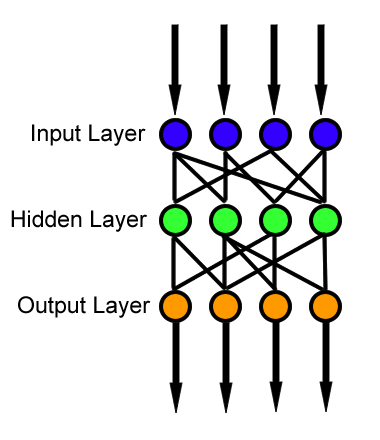
\includegraphics[width=0.4\textwidth]{abb/Feed_forward_neural_net.png}
 \captionof{figure}{Beispiel eines Feed Forward KNNs}
\end{center}


KNNs existieren in zwei Zuständen der Trainingsphase
und der Arbeitsphase. 
Die Trainingsphase ist die interessantere und wird in
dieser Arbeit beleuchtet. Hier werden durch Optimierung 
der Fehlerfunktion die Neuronen so "eingestellt" ,
dass sie einen möglichst gute Vorhersage treffen. 

Im Folgenden soll nun der Begriff des Neurons formalisiert 
werden, um die Verbesserungsmöglichkeiten des Gradienten
Verfahrens in Abschnitt \ref{Optimisierungsmethoden} 
nachvollziehen zu können.

\begin{definition}
\cite[Kapitel 1.2]{BurkhardLenze.1997} Ein (\textbf{formales) Neuron} ist eine Funktion $\kappa: \mathbb{R}^n \rightarrow \mathbb{R}^m$ definiert durch:
\begin{itemize}
\item eine Aktivierungsfunktion $T:\mathbb{R} \rightarrow \mathbb{R}$
\item ein gewichteter Vektor $\vec{w} = \{w_1,w_2,...,w_n\}$
\item und eine Schwelle  $\Theta\in\mathbb{R}$.
\end{itemize}
Der Vektor $\vec{x} = (x_1,x_2,...,x_n)\in \mathbb{R}^n$ wird auf den Vektor $\vec{y} = (y,y,...,y)\in \mathbb{R}^m$ mit identischen Komponenten durch die folgende Rechenvorschrift abgebildet
\begin{align}
\kappa(\vec{x}):= (T(\sum\limits_{i=1}^n w_i x_i - \Theta),...,T(\sum\limits_{i=1}^n w_i x_i - \Theta))=\vec{y} \in \mathbb{R}^m
\end{align}   
\end{definition}
Hier seien ein paar Beispiele für Aktivierungsfunktionen angegeben
\begin{itemize}
\item Identität $T_I$
\begin{align*}
T(x):=x=T_I(x)
\end{align*}
\item Binary step
\begin{align*}
T(x) := \begin{cases} 0, \text{ for } x < 0 \\ 1, \text{ for } x \geq 0 \end{cases} =: T_1 (x)
\end{align*}
\item Sigmoid
\begin{align*}
T(x) := \frac{1}{1+e^{-x}} =: T_S(x)
\end{align*}
\item Tangens hyperbolicus
\begin{align*}
T(x) := \frac{1+tanh(x)}{2} =: T_H(x)
\end{align*}
\end{itemize}
Dies sind nur ein paar wenige Beispiele.
Jede Funktion $T:\mathbb{R}\rightarrow \mathbb{R}$
die $\lim\limits_{x \rightarrow -\infty}{T(x)}=0$ 
and $\lim\limits_{x \rightarrow \infty}{T(x)}=1$ erfüllt,
kann als Aktivierungsfunktion genutzt werden.

\begin{definition}
    \cite[Kapitel 2]{MichaelNielsen.Juni2019}
    Die \textbf{Fehlerfunktion} $J(\theta)$ eines Neuronalen Netzes ist eine 
    differenzierbare Funktion für die gilt:
    \begin{itemize}
        \item $J(\theta) = \frac{1}{n} \sum_x J_x$ wobei $x$ ein Eingabe Datum
        beschreibt.
        \item $J(\theta)$ lässt sich aus der Summe der Elemente des Ausgabe Vektors
        darstellen.
    \end{itemize}
\end{definition}

Die erste Eigenschaft bedeutet, dass die gesamte Fehlerfunktion 
sich auch durch die Fehlerfunkton der einzelnen Eingabe Daten darstellen lässt.
Diese Fehlerfunktion wird im nächsten Abschnitt minimiert werden, um
eine optimale Parameterbelegung der Gewichte $\vec{w}$ zu finden. 
Beispiele für eine solche Funktion wäre der 
mittlere quadratische Fehler.

\subsection{Gradient Descent}\label{Gradient Descent}

Der Gradient Descent oder zu Deutsch Gradienten Abstiegsverfahren
ist ein Weg eine Zielfunktion $J(\theta)$ parametrisiert durch $\theta \in \mathbb{R}^n$
zu minimieren. Man aktualisiert diese Parameter in Richtung des Gradienten
der Zielfunktion $\nabla_\theta J(\theta)$. Die Lern Rate $\mu$ bestimmt
dabei die Größe der Aktualisierungsschritte. Das Verfahren folgt 
also der Richtung des Abstiegs der Oberfläche der Zielfunktion in ein Tal,
welches ein lokales Minimum
beschreibt. \cite{Ruder.9152016} 
Im Fall eines neuronalen Netzes ist die Zielfunktion $J(\theta)$ die
Fehlerfunktion des neuronalen Netzes. 

Das Standard Gradient Descent Verfahren ist das Batch Gradient Descent Verfahren.



\subsection{Optimisierungsmethoden}\label{Optimisierungsmethoden}

\subsubsection{Stochastic Gradient Descent}\label{Stochastic Gradient Descent}

\subsubsection{Adagrad}\label{Adagrad}

\subsubsection{Adam}\label{Adam}